\documentclass[10pt,letterpaper]{article}
\usepackage{ccn}
\usepackage[T1]{fontenc}
\usepackage{amsmath,amssymb,graphicx,booktabs}
\usepackage[round,authoryear]{natbib}
\usepackage[hidelinks]{hyperref}
\usepackage{microtype}
\title{Actionability as an Explanation of Grid Cells:\\A Critical Review of Dorrell et al. (2023)}
\author{{\large\bf Tafara Chibanda (2683459)}\\University of the Witwatersrand
\And {\large\bf Nathan Le Roux (2717495)}\\University of the Witwatersrand}
\begin{document}
\maketitle

\section{Summary}
\citet{dorrell2023} ask why spatial representations should take the form of grid cells: neurons whose firing fields repeat on a hexagonal lattice. Their proposal is that a useful representation must preserve the consequences of actions. Moving by a given displacement should update neural activity through the same linear transformation wherever the movement begins. Combining this \emph{actionability} requirement with non-negative, bounded activity and an objective that separates distinct locations produces grid-like codes in their simulations. Representation theory restricts the code to combinations of spatial waves; the authors then explain how the other constraints favour frequency lattices and, in suitable regimes, hexagonal grids and multiple modules. Predictions concern field width, relative module orientation, and adaptation to room geometry. The paper's central contribution is an interpretable account of why these representations may be useful, rather than a detailed circuit or learning mechanism.

\section{Originality}
Earlier continuous-attractor models explained grid activity and velocity integration \citep{burak2009}, while task-trained networks produced grid-like units for navigation \citep{banino2018}. More directly, \citet{gao2021} already connected path integration to group representations and linear transformations, alongside isotropic scaling. Neither grid formation nor the group-theoretic perspective is therefore entirely new. Dorrell et al.\ combine actionability with functional and biological constraints to explain several features, including modules, without the additional isotropy constraint (Appendix H). This unification is the distinctive contribution.

This is a more abstract approach than specifying synaptic connectivity or training a complete navigating agent. Its advantage is that it separates a computational requirement from a particular implementation: several circuits could realise the same useful code. The framework also extends beyond planar position to variables with other transformation groups. However, it is not more general in every respect. Requiring a location-independent \emph{linear} action on activity is a substantive restriction; representations that use context-dependent or nonlinear updates are outside the analysed class. Periodic components are therefore partly a consequence of the chosen mathematical formulation, even though hexagonal organisation is not directly imposed.

The claim of \emph{minimal constraints} is best read as applying to this modelling framework. The ablations in Appendix I strengthen the argument that the chosen ingredients matter within it. They do not establish that these are the uniquely necessary assumptions across all possible neural mechanisms. The paper would be stronger if this distinction were made as prominent as the unifying claim.

\section{Clarity}
The progression from angular representations to two-dimensional space is effective. It gives the reader a concrete interpretation of actionability before introducing the more demanding representation-theoretic argument. Figure 4 is particularly helpful: the frequency-space explanation connects the two spatial lengthscales to the preference for a hexagonal lattice. Figure 5 then separates the model's predictions into identifiable experimental questions. These illustrations make the mathematical framework more accessible.

Some practical details are harder to reconstruct. Figure 8 describes the spatial-resolution comparison, while the principal parameter table in Appendix B.3 concerns Figure 2B; Appendix B.4 notes further adjustments to optimisation settings. A configuration file for each figure would make the chain from equations to results easier to follow. There is also a potentially consequential distinction between the main-text integral normalisation and the sampled sum in equation 22: the numerical scale of neural distances, and therefore of $\sigma$, depends on the convention.

The public code helps, but does not resolve every ambiguity. In the \href{https://github.com/WilburDoz/ICLR_Actionable_Reps/blob/940659ed2773f4cbb3bcf298bdb70497b30d250c/NRT_functions/losses.py}{inspected version (commit 940659e)}, the norm routine forms normalised responses and subsequently aggregates unnormalised responses, whereas equation 25 uses normalised responses. Its \texttt{sigma\_sq} argument also needs to be distinguished from the paper's $\sigma$. These observations call for clarification of the exact figure-generating setup, rather than a conclusion that the reported results are wrong.

\section{Quality}
A major strength is the combination of analytic reasoning, numerical optimisation, and biological predictions. The frequency-space account explains why non-negativity, location discrimination, and actionability can interact to produce structured codes. The parameter studies and ablations go beyond presenting a single attractive firing map. The authors also acknowledge limitations, including firing-field intensity variation and distortions in irregular environments.

The account of modules is particularly useful. Harmonic components help individual neurons construct non-negative, peaked responses, while harmonically unrelated frequencies help a population distinguish locations that would otherwise share a code. Modules provide a way to accommodate both demands. This connects a population-level objective to single-cell tuning, although the numerical evidence for several clean hexagonal modules is less robust in some parameter regimes, as Appendix B.4.2 acknowledges.

The abstraction is appropriate for asking what makes a representation useful. It is less sufficient for explaining how a rodent learns and maintains that representation. The optimiser has access to position samples and an explicitly specified objective; the paper does not demonstrate a biologically local learning rule or noisy velocity integration in a circuit. Boundedness and non-negativity are reasonable biological constraints, but they do not specify spiking variability, sensory correction, or connectivity. Accordingly, obtaining an optimal code does not establish that an animal can learn it or use it robustly.

The supporting evidence also varies in strength across claims. The mathematical restrictions on admissible codes are more direct than the claim that hexagonal grids globally minimise the full objective. Several lattice arguments are heuristic, and Appendix G acknowledges the non-convex frequency-selection problem and the need for further tools to prove optimality. The simulations support a plausible explanation, rather than a general certificate of the optimum. Appendix B.4 also distinguishes optimisation parameters from parameters defining the objective. That distinction is useful theoretically, but practical reliability still matters when simulation is used as evidence. Reporting distributions across initialisations, constraint residuals, and convergence diagnostics alongside the maps would clarify this boundary.

Finally, the comparisons with biological data are encouraging rather than decisive. The authors describe several as rudimentary. For example, the relationship between field width and recorded cell counts depends on assumptions about sampling neurons across modules. Agreement in a qualitative trend cannot by itself distinguish the proposed explanation from alternatives. Our contrasting reproduction outcomes, described below, reinforce the need for numerical clarity but does not refute the theoretical argument.

\section{Significance}
The strongest prospective contribution is a set of interpretable links between representational demands and measurable neural organisation. This complements circuit models: the theory proposes which codes are useful, while mechanistic models can investigate whether plausible networks can implement them. Recordings showing toroidal population structure in grid-cell modules \citep{gardner2022} make this relationship between population geometry and neural dynamics especially relevant. Such evidence is compatible with the framework, but does not uniquely verify its objective.

A concrete theory--experiment loop follows from the prediction about room geometry. Record the same modules in an arena before and after a controlled change in aspect ratio, measure occupancy, and predict how field spacing and orientation should change under the model. Fit any free parameters using the original environment and assess predictions in the changed environment, rather than refitting each condition. The paper predicts that some codes can remain stable when they are suitable for both geometries, while others should adjust. Comparing that pattern with a competing model would be more informative than checking whether both produce grids.

A useful refinement would separate changes in physical boundaries from changes in sampled occupancy, because the theory expresses environmental effects through $p(x)$. Persistent disagreement after accounting for occupancy would motivate adding sensory anchoring or learning-history effects. This would allow experiments to modify the assumptions of the model, completing the loop. The present work offers valuable hypotheses for this process; it does not yet provide a validated account of all environmental responses.

\section{Reproducibility}
We independently implemented the Fourier model and sampled losses in equations 22--25, using JAX (Tafara) and NumPy (Nathan). On identical float64 inputs, the three unweighted losses agree within $3\times10^{-13}$. After aligning the different functional-loss weights, directional derivatives agree with an independent finite-difference reference within $6\times10^{-11}$. Tests also check translations and checkpoint continuation. These checks support the equations, but cannot certify convergence or equivalence of the training procedures.

Tafara tested the Figure 8 spatial-scale prediction with $N=64$, 31 frequency pairs, $\sigma=0.4$, and $l=0.5$ versus $0.1$, using 150,000 updates per seed-0 run. The norm target 0.02 was an explicit implementation choice, not a reported Figure 8 setting. Both populations showed elongated periodic patterns rather than a clean hexagonal baseline (Figure~\ref{fig:results}); median descriptive scores were 0.0503 and 0.00884. Mean negativity penalties passed their tolerance although 3.61\% and 5.08\% of sampled rates remained below $-10^{-6}$. The $l=0.5$ run also missed the norm target (Table~\ref{tab:results}). These single-seed outcomes do not establish the predicted dependence on $l$.

Nine further 150,000-step runs compared baseline, $\sigma=\sqrt{0.4}$, and norm target $\exp(4)$ over three matched seeds. Changing sigma modestly increased descriptive scores without establishing a hexagonal baseline. Relaxing the norm target increased held-out norm errors to 1.77--3.87 from baseline's 0.0209--0.0301. None met both original tolerances (Figure~\ref{fig:diagnostics}). This is a sensitivity study of specified numerical choices, not an exact rerun of the authors' setup.

Nathan's results provide a contrasting outcome (Table~\ref{tab:joint}). His two 150,000-step runs at $\sigma=1.0$ each produced one module satisfying his stated geometric criteria; analytic grid scores exceeded 0.3 for all cells. At $\sigma=0.2$, none of three full runs met the module criteria. At $\sigma=0.4$, two 50,000-step seeds gave opposite outcomes. His functional weight, initialisation, norm target and Adam convention differ from Tafara's. Thus these are positive geometry examples and evidence of sensitivity, rather than a controlled ranking of implementations. The accompanying code preserves both implementations and their configurations.

Analysis choices matter too. Nathan uses spectral autocorrelation with windows scaled to spatial period; Tafara uses finite-window Pearson autocorrelation. Re-evaluating five Nathan checkpoints with Tafara's common grid and held-out samples gave norm errors of 1.85--5.83. The broad hexagonal examples nevertheless received negative median finite-window scores: the small window contains too few repeats to assess their geometry reliably. Scores are descriptive, without shuffled significance tests, and neurons are not independent repetitions. We also corrected an initially undersampled grid in Tafara's analysis using the learned frequencies, without changing training results.

Finally, our tolerance itself needs calibration. A constructed non-negative hexagonal code with nearly invariant exact Gaussian room energy (relative deviation below $7.2\times10^{-8}$ in tested rooms) had mean sampled norm penalties 0.0961, 0.0274 and 0.00644 at 50, 150 and 600 points over 128 batches (Figure~\ref{fig:control}). Finite sampling can therefore penalise valid geometry under our 0.02 target. This control is not learned evidence or proof of why training failed. Together, the positive and negative results support the paper's geometric possibility while showing why figure-specific settings, constraint calibration and explicit analysis scales are needed for a convincing reproduction.

\begin{thebibliography}{5}
\bibitem[Dorrell et al.(2023)]{dorrell2023}
Dorrell, W., Latham, P. E., Behrens, T. E. J., \& Whittington, J. C. R. (2023).
Actionable neural representations: Grid cells from minimal constraints.
\emph{International Conference on Learning Representations}.
\url{https://arxiv.org/abs/2209.15563}
\bibitem[Burak and Fiete(2009)]{burak2009}
Burak, Y., \& Fiete, I. R. (2009).
Accurate path integration in continuous attractor network models of grid cells.
\emph{PLoS Computational Biology, 5}(2), e1000291.
\url{https://doi.org/10.1371/journal.pcbi.1000291}
\bibitem[Banino et al.(2018)]{banino2018}
Banino, A., Barry, C., Uria, B., et al. (2018).
Vector-based navigation using grid-like representations in artificial agents.
\emph{Nature, 557}, 429--433.
\url{https://doi.org/10.1038/s41586-018-0102-6}
\bibitem[Gao et al.(2021)]{gao2021}
Gao, R., Xie, J., Wei, X.-X., Zhu, S.-C., \& Wu, Y. N. (2021).
On path integration of grid cells: Group representation and isotropic scaling.
\emph{Advances in Neural Information Processing Systems, 34}.
\url{https://arxiv.org/abs/2006.10259}
\bibitem[Gardner et al.(2022)]{gardner2022}
Gardner, R. J., Hermansen, E., Pachitariu, M., Burak, Y., Baas, N. A., Dunn, B. A., Moser, M.-B., \& Moser, E. I. (2022).
Toroidal topology of population activity in grid cells.
\emph{Nature, 602}, 123--128.
\url{https://doi.org/10.1038/s41586-021-04268-7}
\end{thebibliography}

\section{Contribution statement}
Tafara Chibanda (2683459) developed the JAX reproduction, matched-seed diagnostics, equation comparison and sampling-calibration control. Nathan Le Roux (2717495) developed the independent NumPy reproduction, parameter sweeps, ablations and module analysis. The report brings these results together while preserving their distinct numerical conventions.

\section{AI assistance disclosure}
OpenAI Codex assisted with literature checking, implementation, tests, analysis, and drafting this review. Both authors have reviewed and agreed with the review's judgements and confirmed their contributions. The required Faculty AI declaration is supplied separately by the authors.

\clearpage
\onecolumn
\section{Appendix: Evidence for the reproduction section}
\begin{table}[h]
\centering
\caption{Final seed-0 checkpoints after 150,000 steps. Constraint measurements use eight held-out batches. Tolerances are $\exp(-9)$ for the mean negative-activity penalty and 0.02 for the norm loss; the latter is our implementation choice. These are descriptive single-run results.}
\label{tab:results}
\begin{tabular}{lrr}
\toprule
Measurement & $l=0.5$ & $l=0.1$\\
\midrule
Median descriptive grid score & 0.0503 & 0.00884\\
Mean negative-activity penalty & 0.0000996 & 0.0001106\\
Mean squared shifted-room norm error & 0.03011 & 0.01950\\
Mean negativity target met & Yes & Yes\\
Norm target met & No & Yes\\
Sampled rates below $-10^{-6}$ & 3.61\% & 5.08\%\\
\bottomrule
\end{tabular}
\end{table}
\begin{figure}[h]
\centering
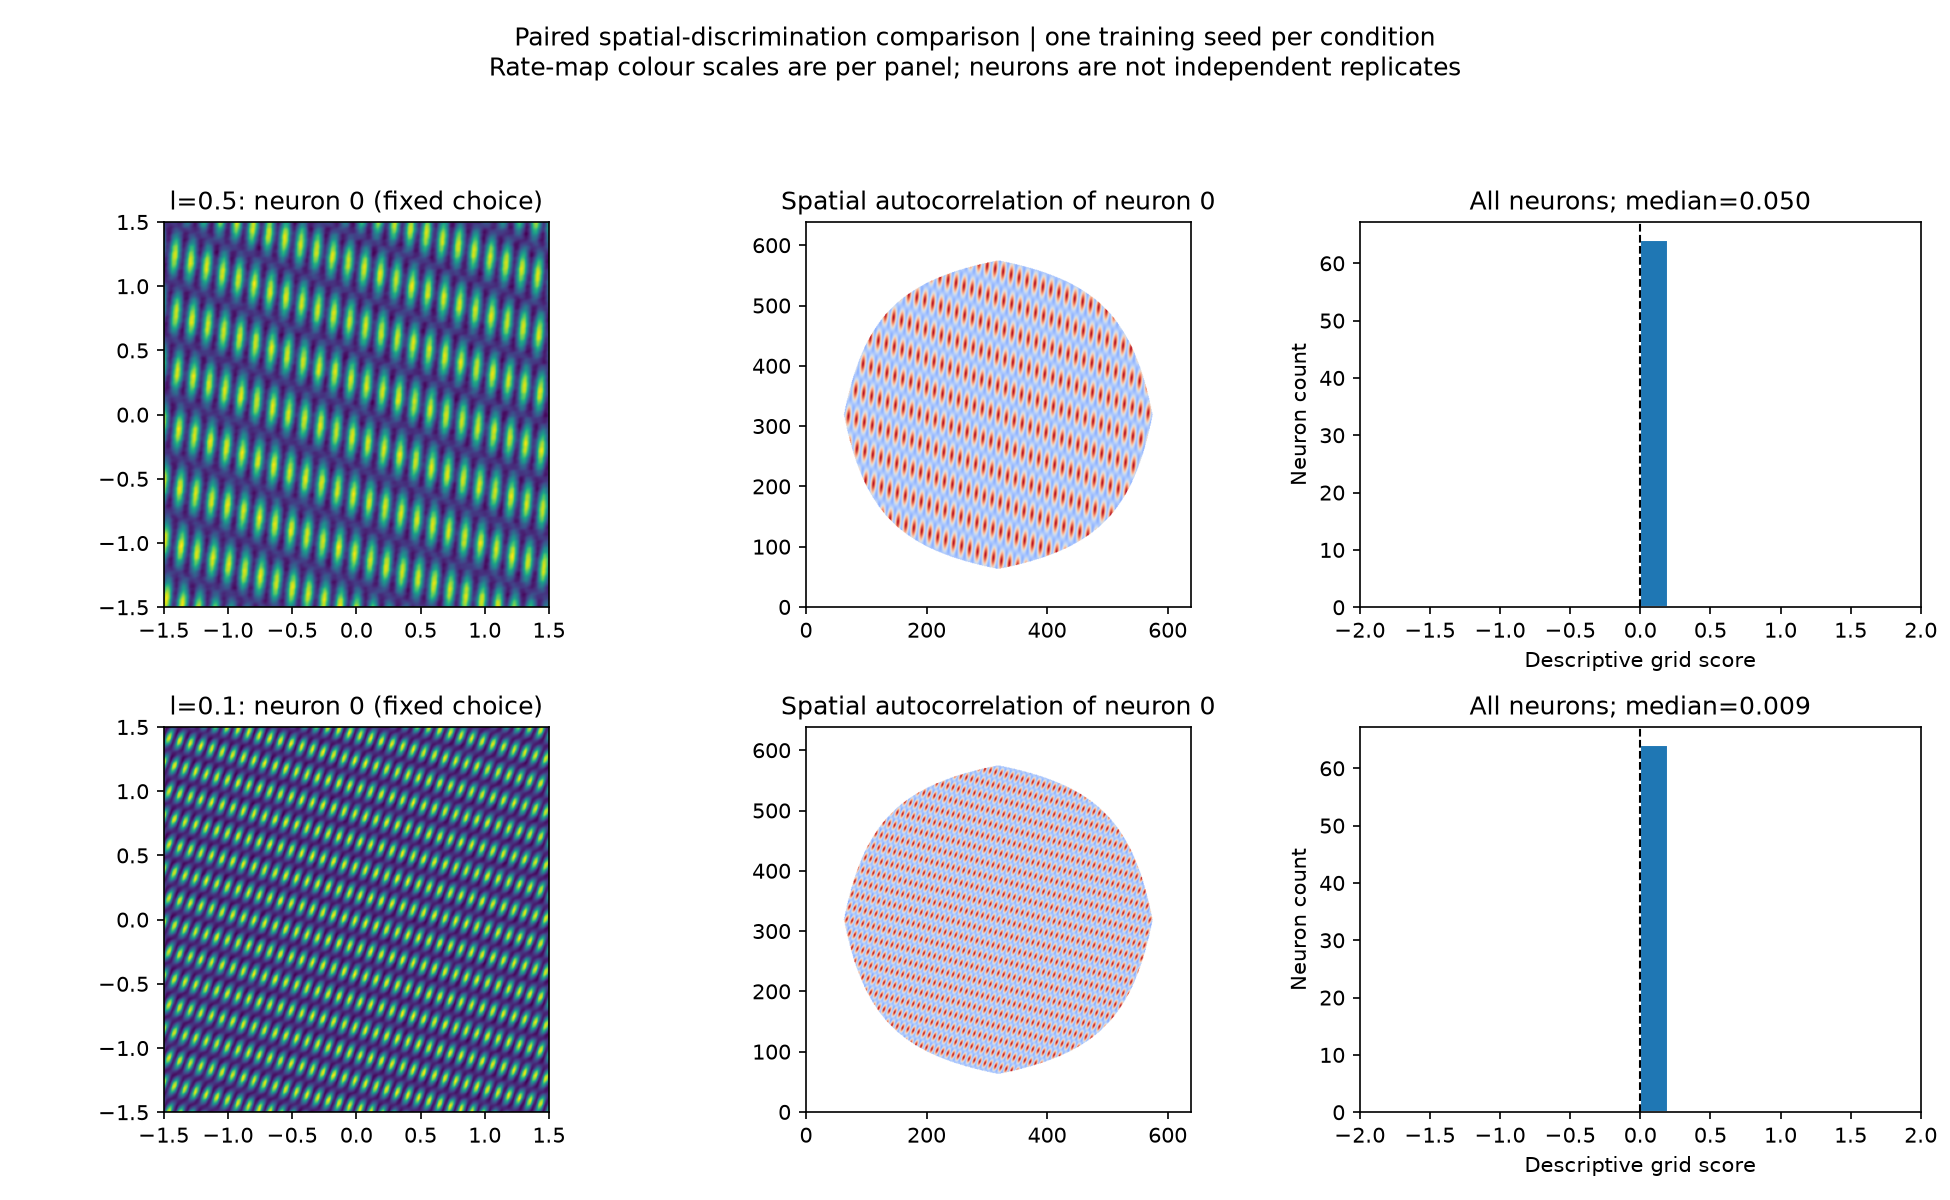
\includegraphics[width=0.95\linewidth]{images/comparison.png}
\caption{The two completed reproduction runs. Neuron 0 is shown by a fixed index choice, with its spatial autocorrelation and the distribution of scores across all 64 neurons. The elongated periodic patterns and near-zero median scores do not establish a hexagonal baseline. Rate-map colour scales differ between panels. Maps use 320 samples per axis over $[-1.5,1.5]^2$; the evaluator checks that learned frequencies are resolved.}
\label{fig:results}
\end{figure}
\clearpage
\section{Appendix: Controlled diagnostics and calibration}
\begin{figure}[h]
\centering
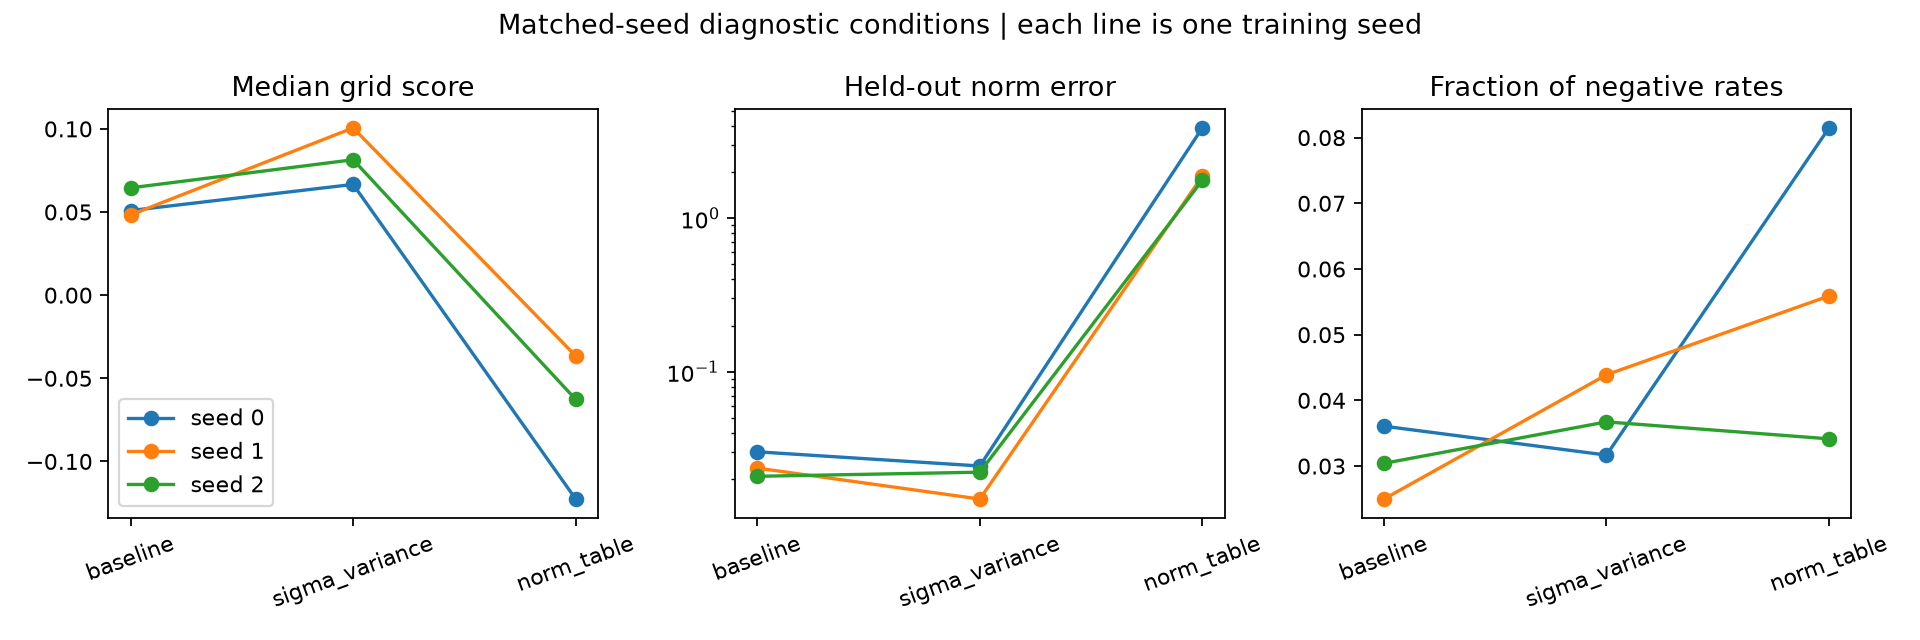
\includegraphics[width=\linewidth]{images/diagnostics.png}
\caption{All nine final checkpoints, each trained for 150,000 steps. Lines connect matched seeds; initial states are identical within each seed. Only the named setting changes: baseline uses $\sigma=0.4$ and norm target 0.02; sigma\_variance uses $\sigma=\sqrt{0.4}$; norm\_table uses norm target $\exp(4)$. All evaluations use the same 352-by-352 grid over $[-1.5,1.5]^2$ and held-out samples. Negative rates are those below $-10^{-6}$. The norm axis is logarithmic. Descriptive grid scores have no shuffled significance calibration. The relaxed-target condition is not a full rerun of the authors' public code.}
\label{fig:diagnostics}
\end{figure}
\begin{figure}[h]
\centering
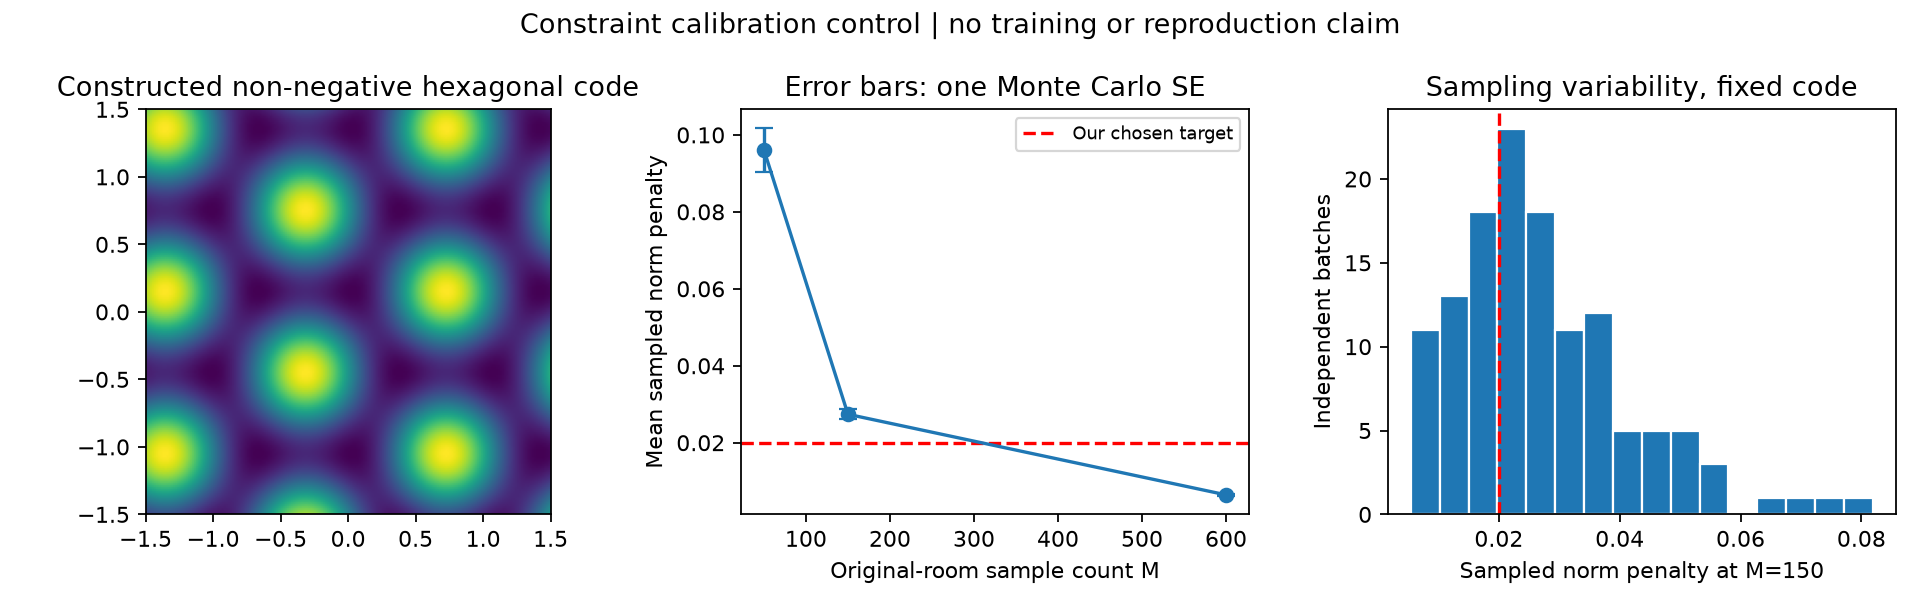
\includegraphics[width=\linewidth]{images/constraint_control.png}
\caption{The constructed-code check discussed in the reproduction section. Left: one fixed-index neuron from a deliberately constructed, non-negative hexagonal population; no training is involved. Centre: the sampled norm penalty decreases with the number of positions used to estimate room energy. Error bars are one standard error across 128 independent sampling batches for the fixed code. Right: the distribution at 150 points shows why our chosen 0.02 threshold can be exceeded even with valid geometry. These sampling batches are not independent training seeds.}
\label{fig:control}
\end{figure}
\clearpage
\section{Appendix: Independent implementation comparison}
\begin{table}[h]
\centering
\caption{Nathan's completed runs from commit df44d69. Module classification requires analytic grid score $>0.3$, six-peak angular error $<15^\circ$ and radial spread $<25\%$. These are descriptive criteria, not shuffled significance tests. Runs within each row share the stated settings; rows do not constitute a matched comparison with Tafara's optimiser.}
\label{tab:joint}
\begin{tabular}{lrrl}
\toprule
Setting & Seeds & Updates per run & Hexagonal modules per seed\\
\midrule
$\sigma=1.0$, $l=0.5$ & 0, 1 & 150,000 & 1, 1\\
$\sigma=0.2$, $l=0.5$ & 0, 1, 2 & 150,000 & 0, 0, 0\\
$\sigma=0.4$, $l=0.5$ & 0, 1 & 50,000 & 1, 0\\
\bottomrule
\end{tabular}
\end{table}
\begin{table}[h]
\centering
\caption{Common evaluation of five Nathan checkpoints. All use eight held-out batches (seed 12345), sum normalisation, and a 352-by-352 map over $[-1.5,1.5]^2$, matching Tafara's diagnostic evaluation. The norm tolerance 0.02 is Tafara's assessment choice; Nathan trained with $\exp(4)$. Small-window scores do not reliably capture broad grid structure, so negative scores here do not negate the spectral geometry results above.}
\begin{tabular}{lrrr}
\toprule
Checkpoint & Median grid score & Norm loss & Mean negativity\\
\midrule
$\sigma=0.2$, seed 0, 150k & 0.0238 & 5.8261 & 0.0001878\\
$\sigma=1.0$, seed 0, 150k & -0.0969 & 3.1925 & 0.0001943\\
$\sigma=1.0$, seed 1, 150k & -0.1907 & 2.6302 & 0.0000858\\
$\sigma=0.4$, seed 0, 50k & -0.0809 & 2.5480 & 0.0000770\\
$\sigma=0.4$, seed 1, 50k & -0.0414 & 1.8502 & 0.0001619\\
\bottomrule
\end{tabular}
\end{table}
\clearpage
\section{NeurIPS checklist: reproduction submission}
\noindent Answers apply to our reproduction, not to Dorrell et al.'s paper. The questions below are abbreviated and paraphrased from the \href{https://neurips.cc/public/guides/PaperChecklist}{NeurIPS checklist}. Author-dependent declarations remain unconfirmed.
\begin{enumerate}
\item \textbf{Are the claims supported and appropriately scoped? Yes.} The review distinguishes the paper's claims, our limited reproduction, and proposed follow-up work. No successful hexagonal baseline is claimed.
\item \textbf{Are limitations explained? Yes.} The reproduction section reports one seed per original spatial-scale condition, three matched seeds in the diagnostic study, numerical departures, unmet constraints, and descriptive rather than inferential grid scores.
\item \textbf{Are new theoretical claims proved? N/A.} We introduce no new theorem; the reviewed theory is attributed to Dorrell et al.
\item \textbf{Can the numerical findings be checked? Yes.} Saved initial/final checkpoints, configurations, metadata, evaluation summaries, and tests accompany the code. Reproduction instructions are in the repository README.
\item \textbf{Are code, inputs, and instructions available? Yes.} The branch \href{https://github.com/TafaraC/NeuroProject/tree/codex/independent-reproduction}{codex/independent-reproduction} contains the original implementation and results. Synthetic positions are generated from recorded seeds; no external dataset is required. Include the updated source with the submission.
\item \textbf{Are experimental choices documented? Yes.} The reproduction section and \texttt{references/implementation\_notes.md} identify the sampling scheme, budget, optimiser, targets, and deviations. Configurations accompany each checkpoint.
\item \textbf{Is uncertainty quantified statistically? No, not for the trained models.} The spatial-scale comparison has one seed per condition; all three seed outcomes are shown for the diagnostics without inferential intervals. Neurons are not treated as independent runs. The constructed control reports sampling standard errors across 128 batches, not training uncertainty.
\item \textbf{Are computing requirements fully reported? No.} The original CPU runs each took approximately 9.3 minutes concurrently; the nine diagnostic training durations sum to 71.2 minutes across processes with two workers. Software and hardware metadata are saved. Peak memory, evaluation cost and total preliminary compute were not fully measured.
\item \textbf{Have the authors confirmed compliance with the ethics code? No; pending author confirmation.} This draft cannot attest that both students have read the code. No new human or animal experiment was conducted.
\item \textbf{Are application-specific societal risks discussed? N/A.} This is a small synthetic modelling exercise without a deployed application or personal data. Its immediate risk is scientific overinterpretation, addressed through explicit limits on claims.
\item \textbf{Are special release safeguards required? N/A.} The released artefacts are a small spatial representation model and synthetic numerical results.
\item \textbf{Are all asset permissions and licences verified? No.} Sources are credited and the model code was independently written, but a complete dependency/licensing audit and a repository redistribution licence remain outstanding before an upstream contribution. The course template is used for its supplied purpose.
\item \textbf{Are newly released artefacts fully documented? No.} Methods, configurations, checkpoints, and limitations are documented; redistribution licensing is still unresolved.
\item \textbf{Are human-participant instructions and compensation described? N/A.} No participants or crowdworkers were recruited.
\item \textbf{Was participant ethics approval obtained where needed? N/A.} No human-subject research was performed, and no new animal data were collected.
\item \textbf{Is substantive LLM assistance disclosed? Yes.} The AI assistance disclosure identifies assistance with code, analysis, literature checking, and drafting. The signed institutional form must still be completed by the authors.
\end{enumerate}

% Tafara will append the completed official Wits Science Faculty AI Declaration here.
% This file is included at the end of main.tex. It intentionally adds no blank page.
% For a completed PDF, add \usepackage{pdfpages} to the main preamble, then:
% \clearpage
% \includepdf[pages=-]{signed_ai_declaration.pdf}
% Alternatively paste the declaration's LaTeX here after \clearpage.

\end{document}
